
\subsection{COMPROBACIÓN DE LOS RESULTADOS}

Como se ha mencionado anteriormente, el trabajo consta de una gran cantidad de
puntos que han sido trabajado de forma modular, esto ha sido con la finalidad
de maximizar la escalabilidad y de facilitar al máximo posible el realizar pruebas
a los módulos y a los acoples realizados. Al momento de comprobar los realizados
se deben de tomar en consideración 2 factores, los resultados técnicos, es decir
funcionalidades de la aplicación, lo cual como se menciono anteriormente no se
automatizaron por factores tiempo y cantidad de pruebas, y los resultados finales,
es decir la capacidad de la herramienta de facilitar el trabajo, mediante
las paginas generales, especificas y exhaustivas.

\subsubsection{Comprobación de resultados a nivel técnico}

Las fallas internas de los servidores, o de procesos de comunicación
con la base de datos, conllevan a la finalización de la ejecución del proceso
(aplicación) correspondiente; esto se hace para poder reiniciar el sistema y
agregar el error o falla catastrófica a un archivo (log) que sirve para seguir el
comportamiento del servidor.

En el caso del servidor de sensorica, estos errores son manejados de forma manual
y se utiliza la característica de Go ``panic" para detener la ejecución, mas
específicamente un paquete de la librería estándar ``log" con la función ``log.Faltalf",
por otro lado, el Framework de Django se encarga de esto, si el error es manejable,
algún problema en una petición o algo no catastrófico, arroja una excepción y un
error 500, fallo interno en el servidor, y finaliza la petición; en el caso de no
poder ser recuperado finaliza el proceso.

La finalización del servidor es una practica relativamente común ya que permite
el reinicio del proceso, esto se hace mediante una configuración interna al
momento de hacer deploy en el servidor, como se observa en la figura \ref{ProcesosLinux}
es la configuración recomendada por DigitalOcean para un reinicio, en caso de falla,
continuo a intervalos de 5 segundos.

	\begin{figure}[htb]
		\centering
        \caption{Configuración de proceso en Linux para reinicio automático de procesos}
        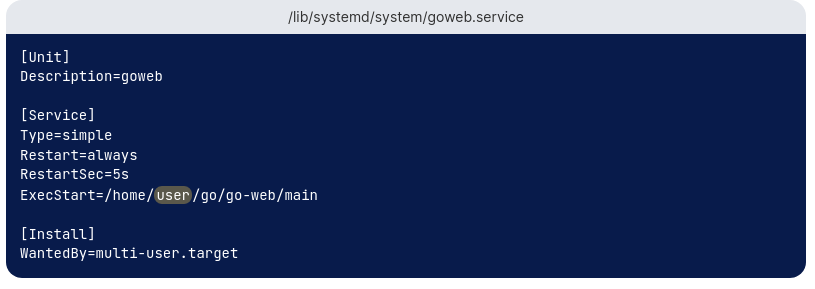
\includegraphics[width=\linewidth]{reinicio_servidor.png}
        Configuración recomendada de \Cite{ConfiguracionProcesos}.
        \label{ProcesosLinux}
	\end{figure}

Por esta razón, las pruebas mas considerables son interconexiones y configuraciones
de seguridad y problemas de datos. es decir:

\begin{itemize}
    \item Prueba de no unicidad de la información, al haber múltiples
        clientes de sensorica enviando información sobre el mismo motor.

        Para esta posibilidad, se opto por una configuración que rechaza el
        segundo intento de conexión, es decir, se rechaza cualquier intento de
        conexión de motor con una conexión establecida previamente (que todavía
        exista), y su implementación se observa en la figura \ref{NoUnicidad}.
%
    \item Prueba de falla en la conexión de la base de datos.

        Cada servidor toma esta falla de una forma especifica, en el caso del
        servidor de sensorica, esta es considerada una falla catastrófica, por
        lo que se finaliza la ejecución, como se observa en la figura
        \ref{NoBBDDSensorica}.

        Por otro lado, el servidor Web arroja una excepción, la cual es manejada
        internamente por Django y resuelta de forma que la petición es respondida
        con un error 500, falla interna del servidor, este error en la respuesta
        dada es manejado por el cliente y se observa en la figura
        \ref{NoBBDDWeb} .
%
    \item Prueba de solicitud de vista exhaustiva a un motor sin conexión
        establecida.

        Este caso corresponde al servidor de sensorica, al no haber una conexión
        con el sensor establecida no se pueden tomar las mediciones para una vista
        exhaustiva, estas deben ser a tiempo real, por lo tanto se responde
        con una error en la respuesta como se observa en \ref{ErrorExhaustiva}.
%
    \item Prueba de petición no completada en el cliente Web,
        información invalida (motor no existente) o error del servidor Web.

        En este caso el cliente muestra un error por pantalla, como ventana
        emergente, y redirige a la vista general, se observa en las figuras y  .
\end{itemize}


	\begin{figure}[htb]
		\centering
        \caption{Prueba de error, no unicidad de información}
        \includegraphics[width=\linewidth]{NoUnicidadSensorica.png}
        logs: Izquierda cliente conectado, Centro cliente Rechazado, Derecha.
        Servidor.
        \label{NoUnicidad}
	\end{figure}

    \begin{figure}[htb]
		\centering
        \caption{Prueba de error, no BBDD Sensorica}
        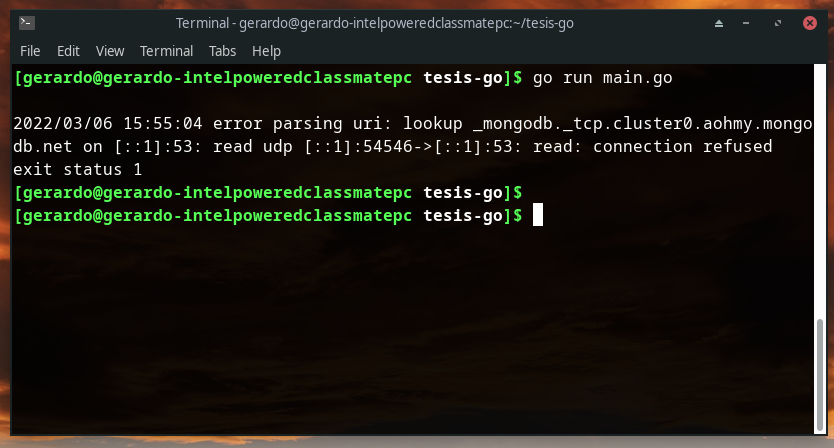
\includegraphics[width=\linewidth]{conexionInvalidaNoBBDDSensorica.png}
        El sistema no inicia por no poder conectarse a la BBDD.
        \label{NoBBDDSensorica}
	\end{figure}

    \begin{figure}[htb]
		\centering
        \caption{Prueba de error, no BBDD Web}
        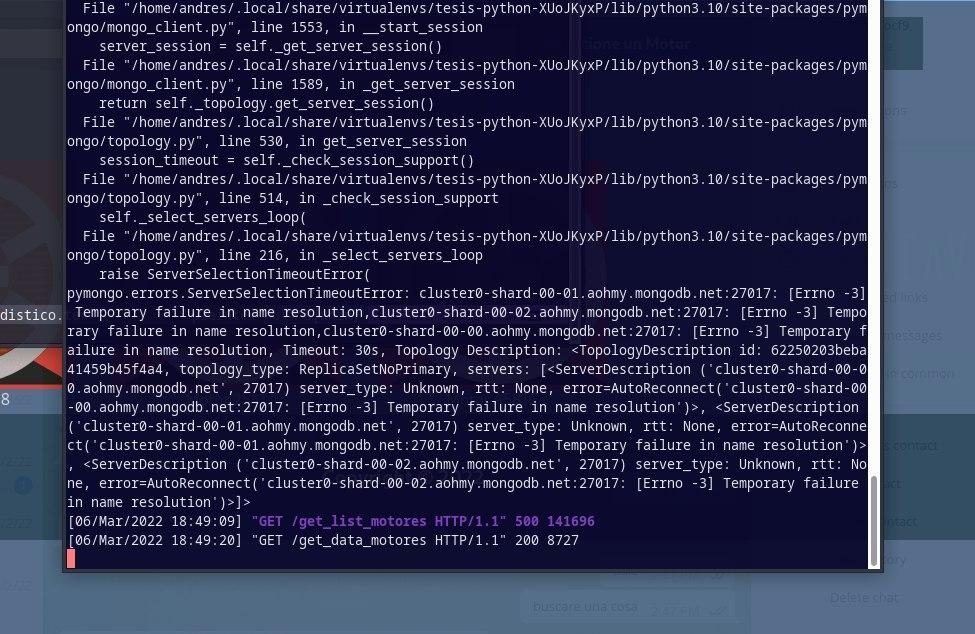
\includegraphics[width=\linewidth]{conexionInvalidaNoBBDDWeb.png}
        El sistema continua ejecución y resuelve el error con un error 500.
        \label{NoBBDDWeb}
	\end{figure}

    \begin{figure}[htb]
		\centering
        \caption{Prueba de error, petición exhaustiva invalida}
        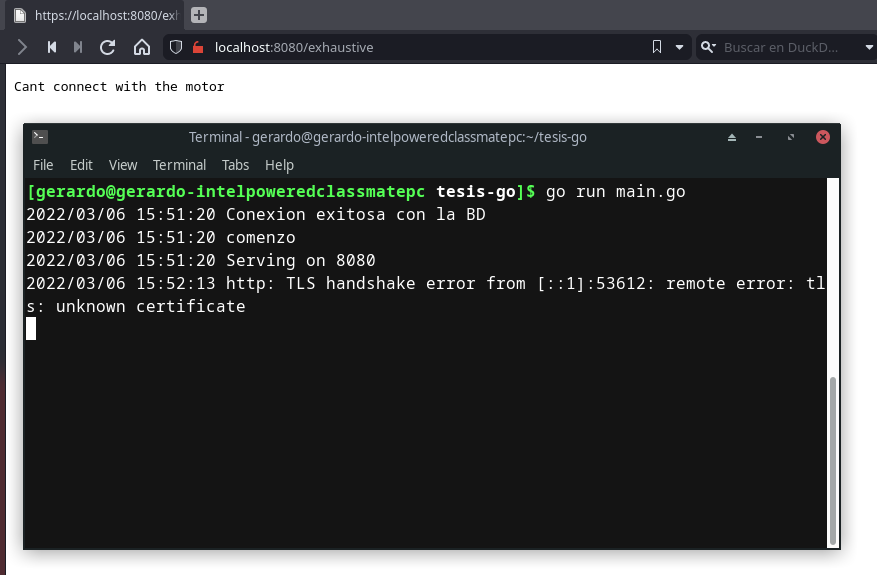
\includegraphics[width=\linewidth]{conexionInvalidaNoMotorSensorica.png}
        Solicitud desde el navegador, para facilitar vista, al servidor
        sin motores conectados.
        \label{ErrorExhaustiva}
	\end{figure}


\subsubsection{Comprobación de resultados finales}
\begin{itemize}
    \item Corroboración del análisis en nivel de daño básico (vista general)
        que se ajuste a los parámetros requeridos por el cliente.
    \item Corroboración de las gráficas históricas.
    \item Corroboración de la gráfica de la transformada de Fourier.
\end{itemize}


